\documentclass[11pt,a4paper]{article}

% --- Essential Typographic & Layout Packages ---
\usepackage[utf8]{inputenc}
\usepackage[T1]{fontenc}
\usepackage[margin=1in]{geometry}
\usepackage{microtype}
\usepackage{amsmath,amssymb,amsthm}
\usepackage{enumitem}

% --- TikZ & Pgfplots for Mathematics Illustrations ---
\usepackage{tikz}
\usepackage{pgfplots}
\pgfplotsset{compat=1.18}

% --- Color & UI Background Packages ---
\usepackage[dvipsnames]{xcolor}
\usepackage[most]{tcolorbox}
\usepackage{hyperref}

% --- Academic Green Design Palette ---
\definecolor{AcademicGreen}{RGB}{20, 82, 40}
\definecolor{DarkGreen}{RGB}{12, 54, 26}
\definecolor{LightGreenBg}{RGB}{242, 248, 244}
\definecolor{BorderGreen}{RGB}{175, 205, 185}
\definecolor{AccentGreen}{RGB}{40, 130, 70}

% --- Hyperlink Setup ---
\hypersetup{
    colorlinks=true,
    linkcolor=AcademicGreen,
    citecolor=AcademicGreen,
    urlcolor=AcademicGreen
}

% --- Custom Header Command ---
\newcommand{\Heading}[1]{\vspace{0.3cm}\noindent\textbf{\textcolor{AcademicGreen}{\large #1}}\par\vspace{0.15cm}}

% --- Custom Box Style ---
\tcbset{
    greenbox/.style={
        colback=LightGreenBg,
        colframe=BorderGreen,
        arc=3mm,
        boxrule=1pt,
        left=10pt, right=10pt, top=8pt, bottom=8pt
    },
    theorembox/.style={
        colback=LightGreenBg,
        colframe=AcademicGreen,
        arc=2mm,
        fonttitle=\bfseries\color{white},
        coltitle=white,
        boxrule=1.2pt,
        left=10pt, right=10pt, top=8pt, bottom=8pt
    }
}

\begin{document}

% ==========================================
% PAGE 1 (Corresponding to Handwritten Page 1)
% ==========================================
\begin{center}
    {\LARGE\bfseries\textcolor{AcademicGreen}{Differential Equations}} \\[0.2cm]
    {\small\textcolor{DarkGreen}{\textbf{Lecture Notes \& Foundations}}}
    \vspace{0.4cm}
\end{center}

\Heading{Differential Equations (DE):}
An equation involving derivatives of one or more dependent variables with respect to one or more independent variables is called a \textbf{differential equation}.

\Heading{Ordinary Differential Equation (ODE):}
A differential equation involving ordinary derivatives of one or more dependent variables with respect to a single independent variable is called an \textbf{ordinary differential equation}.

\Heading{Partial Differential Equation (PDE):}
A differential equation involving partial derivatives of one or more dependent variables with respect to more than one independent variable is called a \textbf{partial differential equation}.

\vspace{0.4cm}
\begin{tcolorbox}[greenbox]
    {\small\textbf{\textcolor{AcademicGreen}{EXAMPLES OF DIFFERENTIAL EQUATIONS}}}
    \vspace{0.2cm}
    \begin{description}[leftmargin=0.4cm, style=nextline, font=\normalfont\bfseries\textcolor{DarkGreen}]
        \item[Ordinary Differential Equations (ODE)]
        \[ \frac{d^2y}{dx^2} + xy\left(\frac{dy}{dx}\right)^2 = 0 \]
        \[ \frac{d^4x}{dt^4} + 5\frac{d^2x}{dt^2} + 3x = \sin(t) \]
        \item[Partial Differential Equations (PDE)]
        \[ \frac{\partial v}{\partial s} + \frac{\partial v}{\partial t} = v \]
        \[ \frac{\partial^2 u}{\partial x^2} + \frac{\partial^2 u}{\partial y^2} + \frac{\partial^2 u}{\partial z^2} = 0 \]
        
        \item[Basic Derivatives (Not Differential Equations)]
        \[ \frac{d}{dx}\left(e^{ax}\right) = ae^{ax} \]
        \[ \frac{d}{dx}(uv) = u\frac{dv}{dx} + v\frac{du}{dx} \]
    \end{description}
\end{tcolorbox}

\newpage

\Heading{Order of a DE:}
The order of the highest-ordered derivative involved in a differential equation is called the \textbf{order} of the differential equation.

\Heading{Degree of a DE:}
The power (or degree) of the highest-ordered derivative involved in a differential equation is called the \textbf{degree} of the differential equation.

\vspace{0.3cm}
\begin{tcolorbox}[greenbox]
    {\small\textbf{\textcolor{AcademicGreen}{CLASSIFICATION BY ORDER AND DEGREE}}}
    \vspace{0.2cm}
    \begin{description}[leftmargin=0.4cm, style=nextline, font=\normalfont\bfseries\textcolor{DarkGreen}]
        \item[2nd Order, 1st Degree ODE]
        \[ \frac{d^2y}{dx^2} + xy\left(\frac{dy}{dx}\right)^2 = 0 \]
        
        \item[4th Order, 1st Degree ODE]
        \[ \frac{d^4x}{dt^4} + 5\frac{d^2x}{dt^2} + 3x = \sin(t) \]
        
        \item[1st Order, 1st Degree PDE]
        \[ \frac{\partial v}{\partial s} + \frac{\partial v}{\partial t} = v \]
        
        \item[2nd Order, 1st Degree PDE]
        \[ \frac{\partial^2 u}{\partial x^2} + \frac{\partial^2 u}{\partial y^2} + \frac{\partial^2 u}{\partial z^2} = 0 \]
        
        \item[2nd Order, 2nd Degree PDE]
        \[ \left(\frac{\partial^2 z}{\partial x^2}\right)^2 + \left(\frac{\partial^2 z}{\partial y^2}\right)^2 = 0 \]
    \end{description}
\end{tcolorbox}

\newpage

% ==========================================
% PAGE 3 (Corresponding to Handwritten Page 3)
% ==========================================

\Heading{Linear ODE:}
A linear ordinary differential equation of order $n$, in the dependent variable $y$ and the independent variable $x$, is an equation that can be expressed in the form:
\[
a_0(x)\frac{d^n y}{dx^n} + a_1(x)\frac{d^{n-1}y}{dx^{n-1}} + \dots + a_{n-1}(x)\frac{dy}{dx} + a_n(x)y = b(x)
\]
where $a_0(x)$ is not identically zero.

\vspace{0.2cm}
\noindent\textbf{\textcolor{DarkGreen}{Key Observations for Linearity:}}
\begin{enumerate}[label=\arabic*), leftmargin=0.6cm, itemsep=0.05cm]
    \item The dependent variable $y$ and its various derivatives occur to the $1^{\text{st}}$ degree only.
    \item No products of $y$ and/or any of its derivatives are present.
    \item No transcendental functions of $y$ or its derivatives occur (e.g., $\sin y$, $e^y$).
\end{enumerate}

\Heading{Nonlinear ODE:}
A non-linear ordinary differential equation is an ordinary differential equation that is not linear.

\vspace{0.3cm}
\begin{tcolorbox}[greenbox]
    {\small\textbf{\textcolor{AcademicGreen}{EXAMPLES OF LINEAR DIFFERENTIAL EQUATIONS}}}
    \vspace{0.2cm}
    \begin{description}[leftmargin=0.4cm, style=nextline, font=\normalfont\bfseries\textcolor{DarkGreen}]
        \item[(a) Linear ODE with Constant Coefficients]
        \[ \frac{d^2y}{dx^2} + 5\frac{dy}{dx} + 6y = 0 \quad \text{Coefficients: } (1, 5, 6) \]
        
        \item[(b) Linear ODE with Variable Coefficients]
        \[ \frac{d^4y}{dx^4} + x^2\frac{d^3y}{dx^3} + x^3\frac{dy}{dx} = xe^x \quad \text{Coefficients: } (1, x^2, x^3) \]
    \end{description}
\end{tcolorbox}

\newpage

% ==========================================
% PAGE 4 (Corresponding to Handwritten Page 4)
% ==========================================

\Heading{Examples of Nonlinear ODEs:}
\begin{enumerate}[label=\arabic*), leftmargin=0.6cm, itemsep=0.2cm]
    \item \[ \frac{d^2y}{dx^2} + 5\frac{dy}{dx} + 6y^2 = 0 \]
    \textit{Reason:} The dependent variable $y$ is raised to the second power ($y^2$), violating linearity.
    
    \item \[ \frac{d^2y}{dx^2} + 5\left(\frac{dy}{dx}\right)^3 + 6y = 0 \]
    \textit{Reason:} The derivative $\frac{dy}{dx}$ is raised to the third power, violating linearity.
    
    \item \[ \frac{d^2y}{dx^2} + 5y\frac{dy}{dx} + 6y = 0 \]
    \textit{Reason:} The dependent variable $y$ and its derivative $\frac{dy}{dx}$ are multiplied together.
\end{enumerate}

\Heading{Origin and Applications:}
Differential equations occur in connection with numerous problems encountered across various branches of science and engineering:
\begin{itemize}[leftmargin=0.5cm, itemsep=0.05cm]
    \item Population Dynamics
    \item Dynamical Systems and Chaos
    \item Fluid Dynamics
    \item Meteorology
    \item Heat Transfer
    \item Biophysics
    \item ...etc.
\end{itemize}

\Heading{Formation of Differential Equations:}
\noindent\textbf{Example Problem:} \\
Form the differential equation from $y = ax + bx^2$ by eliminating the arbitrary constants $a$ and $b$.

\noindent\textbf{Solution:} \\
Given the relation:
\begin{equation}
    y = ax + bx^2 \label{eq:page4_orig}
\end{equation}
Differentiating with respect to $x$:
\begin{equation}
    \frac{dy}{dx} = a + 2bx \implies a = \frac{dy}{dx} - 2bx \label{eq:page4_a}
\end{equation}
Differentiating again with respect to $x$:
\begin{equation}
    \frac{d^2y}{dx^2} = 2b \implies b = \frac{1}{2}\frac{d^2y}{dx^2} \label{eq:page4_b}
\end{equation}
Substituting \eqref{eq:page4_b} into \eqref{eq:page4_a}:
\[ a = \frac{dy}{dx} - x\frac{d^2y}{dx^2} \]
Substituting $a$ and $b$ back into \eqref{eq:page4_orig}:
\[ y = x\left(\frac{dy}{dx} - x\frac{d^2y}{dx^2}\right) + \frac{1}{2}x^2\frac{d^2y}{dx^2} = x\frac{dy}{dx} - \frac{1}{2}x^2\frac{d^2y}{dx^2} \]
Rearranging terms yields the final 2nd order ODE:
\[ x^2\frac{d^2y}{dx^2} - 2x\frac{dy}{dx} + 2y = 0 \]

\newpage

% ==========================================
% PAGE 5 (Corresponding to Handwritten Page 5)
% ==========================================

\Heading{General Solution:}
The relation containing $n$ arbitrary constants which satisfies an ODE of $n^{\text{th}}$ order is called its \textbf{complete primitive} or \textbf{general solution}.

\vspace{0.15cm}
\begin{tcolorbox}[greenbox]
    \textbf{\textcolor{AcademicGreen}{Note:}} It can be shown that, by eliminating $n$ arbitrary constants from an equation in $x$ and $y$, we obtain a differential equation of $n^{\text{th}}$ order. Such a process is called the \textbf{formation of a differential equation}.
\end{tcolorbox}

\Heading{Particular Solution:}
A \textbf{particular solution} is one obtained from the primitive or general solution by assigning definite values to the arbitrary constants.

\Heading{Geometrical Interpretation:}
Geometrically, the primitive represents the equation of a \textbf{family of curves} satisfying the differential equation, and a particular solution represents the equation of \textbf{one member} of this family of curves.

\Heading{Example Problem:}
Form the differential equation from the family of parabolas:
\begin{equation}
    (x - h)^2 = 4a(y - k) \label{eq:parabola_fam}
\end{equation}
where $a, h, k$ are arbitrary constants.

\noindent\textbf{Solution:} \\
Differentiating \eqref{eq:parabola_fam} with respect to $x$:
\begin{equation}
    2(x - h) = 4a \frac{dy}{dx} \implies (x - h) = 2a \frac{dy}{dx} \label{eq:par_diff1}
\end{equation}
Differentiating \eqref{eq:par_diff1} again with respect to $x$:
\begin{equation}
    1 = 2a \frac{d^2y}{dx^2} \implies \frac{d^2y}{dx^2} = \frac{1}{2a} \label{eq:par_diff2}
\end{equation}

\noindent Differentiating \eqref{eq:par_diff2} once more with respect to $x$:
\[
\frac{d^3y}{dx^3} = 0
\]
which is the required differential equation of order 3.

\Heading{Nature of Solutions:}
Consider the general $n^{\text{th}}$ order differential equation:
\begin{equation}
    F\left(x, y, \frac{dy}{dx}, \frac{d^2y}{dx^2}, \ldots, \frac{d^ny}{dx^n}\right) = 0 \label{eq:nth_order}
\end{equation}
where $F$ is a real-valued function of its $(n+2)$ arguments.

\vspace{0.2cm}
\begin{enumerate}[label=\textbf{\arabic*.}]
    \item \textbf{Explicit Solution:} Let $f$ be a real function defined for all $x$ in an interval $I$ and having an $n^{\text{th}}$ derivative for all $x \in I$. The function $f$ is called an \textbf{explicit solution} of the DE \eqref{eq:nth_order} on $I$ if it fulfills the following two requirements:
    \begin{enumerate}[label=\roman*)]
        \item $F\left(x, f(x), f'(x), \ldots, f^{(n)}(x)\right)$ is defined for all $x \in I$.
        \item $F\left(x, f(x), f'(x), \ldots, f^{(n)}(x)\right) = 0 \quad \forall x \in I$.
    \end{enumerate}

    \vspace{0.3cm}
    \item \textbf{Implicit Solution:} A relation $g(x,y) = 0$ is called an \textbf{implicit solution} of the DE \eqref{eq:nth_order} if this relation defines at least one real function $f$ of variable $x$ on $I$ such that this function is an explicit solution of \eqref{eq:nth_order} on $I$.
    \item Both explicit and implicit solutions will usually be called simply \textbf{solutions}.
\end{enumerate}

\Heading{Example 1:}
Show that $f(x) = 2\sin x + 3\cos x$ is an explicit solution of $\frac{d^2y}{dx^2} + y = 0$ for all $x$.

\noindent\textbf{Solution:} \\
Given $f(x) = 2\sin x + 3\cos x$. The derivatives are:
\[ f'(x) = 2\cos x - 3\sin x, \quad f''(x) = -2\sin x - 3\cos x \]
Substituting into the DE:
\[ \frac{d^2y}{dx^2} + y = (-2\sin x - 3\cos x) + (2\sin x + 3\cos x) = 0 \]
This holds for all real $x$. Therefore, $f(x)$ is an explicit solution.

\Heading{Example 2:}
Consider $\frac{dy}{dx} = 2x$. This differential equation has a one-parameter family of solutions:
\[ y = x^2 + c \]
where $c$ is an arbitrary constant (parameter).

\begin{center}
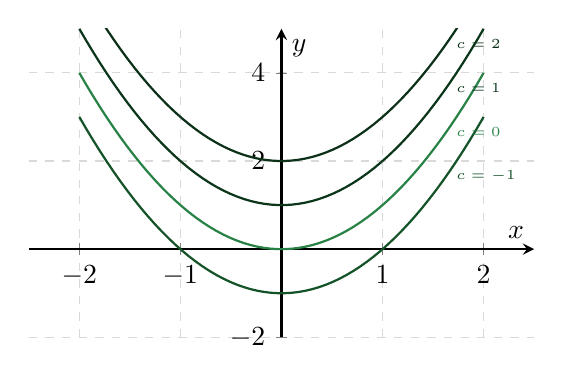
\begin{tikzpicture}
  \begin{axis}[
      axis lines = middle,
      xlabel = {$x$},
      ylabel = {$y$},
      xmin = -2.5, xmax = 2.5,
      ymin = -2, ymax = 5,
      domain = -2:2,
      samples = 60,
      width=8cm, height=5.5cm,
      grid = major,
      grid style = {dashed, gray!30},
      thick
  ]
    \addplot[AcademicGreen, thick] {x^2 - 1} node[pos=0.85, right] {\tiny $c=-1$};
    \addplot[AccentGreen, thick] {x^2} node[pos=0.85, right] {\tiny $c=0$};
    \addplot[DarkGreen, thick] {x^2 + 1} node[pos=0.85, right] {\tiny $c=1$};
    \addplot[AcademicGreen!60!black, thick] {x^2 + 2} node[pos=0.85, right] {\tiny $c=2$};
  \end{axis}
\end{tikzpicture}
\end{center}

\Heading{Exercise:}
Show that $f(x) = c_1 e^{4x} + c_2 e^{-2x}$ is a solution of $y'' - 2y' - 8y = 0$.

\noindent\textbf{Solution:} \\
$f'(x) = 4c_1 e^{4x} - 2c_2 e^{-2x}$ and $f''(x) = 16c_1 e^{4x} + 4c_2 e^{-2x}$.
\[ y'' - 2y' - 8y = (16c_1 e^{4x} + 4c_2 e^{-2x}) - 2(4c_1 e^{4x} - 2c_2 e^{-2x}) - 8(c_1 e^{4x} + c_2 e^{-2x}) = 0 \]
Thus, $f(x)$ is an explicit solution for all real $x$.

\newpage

% ==========================================
% PAGE 8 (Corresponding to Handwritten Page 8)
% ==========================================

\Heading{Initial Value Problem (IVP) \& Boundary Value Problem (BVP)}

\Heading{Example:}
Consider $\frac{dy}{dx} = 2x \quad \text{--- (1)}$ subject to $y(1) = 4 \quad \text{--- (2)}$.

\noindent\textbf{Solution:} \\
Equation (1) has a 1-parameter family of solutions:
\begin{equation}
    y = x^2 + c \label{eq:page8_fam}
\end{equation}
Applying condition (2) by substituting $x = 1$:
\[ y(1) = 1^2 + c \implies 4 = 1 + c \implies c = 3 \]
Thus, $y = x^2 + 3$ is the unique solution of (1) satisfying condition (2).

\Heading{Supplementary Conditions:}
In practical applications of both first and higher-order differential equations, problems involve a DE along with one or more supplementary conditions which the solution must satisfy.

\vspace{0.2cm}
\begin{tcolorbox}[greenbox]
    \textbf{\textcolor{AcademicGreen}{Initial-Value Problem (IVP):}} \\
    If all associated supplementary conditions relate to \textbf{one} single value of $x$, the problem is called an \textbf{initial-value problem} (or one-point boundary value problem).
\end{tcolorbox}

% ==========================================
% PAGE 9 (Corresponding to Handwritten Page 9)
% ==========================================

\begin{tcolorbox}[greenbox]
    \textbf{\textcolor{AcademicGreen}{Boundary Value Problem (BVP):}} \\
    If the supplementary conditions relate to \textbf{two different} values of $x$, the problem is called a \textbf{two-point boundary value problem} or simply a \textbf{boundary value problem}.
\end{tcolorbox}

\Heading{Comparison Examples:}
\begin{description}[leftmargin=0.4cm, font=\normalfont\bfseries\textcolor{DarkGreen}]
    \item[Initial Value Problem (IVP):]
    \[ \frac{d^2y}{dx^2} + y = 0, \quad y(1) = 3, \; y'(1) = 4 \quad \text{(Conditions evaluated at single point } x=1) \]
    
    \item[Boundary Value Problem (BVP):]
    \[ \frac{d^2y}{dx^2} + y = 0, \quad y(0) = 1, \; y\left(\frac{\pi}{2}\right) = 5 \quad \text{(Conditions evaluated at } x=0 \text{ and } x=\frac{\pi}{2}) \]
\end{description}

\vspace{0.3cm}
\begin{tcolorbox}[theorembox, title={Existence and Uniqueness Theorem}]
Consider the first-order differential equation:
\[ \frac{dy}{dx} = f(x, y) \quad \text{--- (*)} \]
where:
\begin{enumerate}[label=\arabic*)]
    \item $f(x, y)$ is a continuous function in some domain $D$ of the $xy$-plane, and
    \item $\frac{\partial f}{\partial y}$ is also a continuous function of $x$ and $y$ in $D$.
\end{enumerate}
Let $(x_0, y_0)$ be an interior point of $D$. Then there exists a \textbf{unique solution} $\phi(x)$ of the DE (*) defined on some interval $|x - x_0| \le h$ (where $h > 0$ is sufficiently small) that satisfies the initial condition:
\[ \phi(x_0) = y_0 \]
\end{tcolorbox}
\textit{Reference: S.L. Ross, Differential Equations, $3^{\text{rd}}$ Edition, p. 21.}

\newpage

% ==========================================
% PAGE 10 (Corresponding to Handwritten Page 10)
% ==========================================

\Heading{Formation of Differential Equations}
\textit{Method: Eliminating ordinary arbitrary constants.}

\Heading{Example 1:}
Form the differential equation by eliminating arbitrary constants $a$ and $b$ from:
\[ y = ax + bx^2 \]

\noindent\textbf{Solution:} \\
Given $y = ax + bx^2 \quad \text{--- (1)}$.
Differentiating once: $\frac{dy}{dx} = a + 2bx \quad \text{--- (2)}$. \\
Differentiating again: $\frac{d^2y}{dx^2} = 2b \implies b = \frac{1}{2}\frac{d^2y}{dx^2} \quad \text{--- (3)}$. \\
From (2): $a = \frac{dy}{dx} - 2bx = \frac{dy}{dx} - x\frac{d^2y}{dx^2} \quad \text{--- (4)}$. \\
Substituting (3) and (4) into (1):
\[ y = x\left(\frac{dy}{dx} - x\frac{d^2y}{dx^2}\right) + \frac{1}{2}x^2\frac{d^2y}{dx^2} \implies x^2\frac{d^2y}{dx^2} - 2x\frac{dy}{dx} + 2y = 0 \]

\Heading{Example 2:}
Form the differential equation of all parabolas whose axes are parallel to the $y$-axis.

\noindent\textbf{Solution:} \\
The general equation of parabolas with vertical axes is given by:
\begin{equation}
    (x - h)^2 = 4a(y - k) \label{eq:vert_parabola}
\end{equation}
where $a, h, k$ are three arbitrary constants.

\noindent Differentiating \eqref{eq:vert_parabola} with respect to $x$:
\[ 2(x - h) = 4a \frac{dy}{dx} \implies (x - h) = 2a \frac{dy}{dx} \]
Differentiating a second time:
\[ 1 = 2a \frac{d^2y}{dx^2} \implies \frac{d^2y}{dx^2} = \frac{1}{2a} \]
Differentiating a third time:
\[ \frac{d^3y}{dx^3} = 0 \]
which is the required differential equation of $3^{\text{rd}}$ order.

\newpage

% ==========================================
% PAGE 1 (Corresponding to Image 1)
% ==========================================
\begin{center}
    {\LARGE\bfseries\textcolor{AcademicGreen}{First Order \& First Degree Differential Equations}} \\[0.2cm]
    {\small\textcolor{DarkGreen}{\textbf{Lecture Notes --- Section 1: Separable Equations}}}
    \vspace{0.3cm}
\end{center}

\Heading{Equations of First Order and 1st Degree:}
The $1^{\text{st}}$ order differential equation can be expressed as:
\begin{align}
    \frac{dy}{dx} &= f(x,y) \quad &\text{--- (i) (Derivative Form)} \label{eq:deriv_form} \\
    \text{or, } M(x,y)dx + N(x,y)dy &= 0 \quad &\text{--- (ii) (Differential Form)} \label{eq:diff_form}
\end{align}
An equation in one of these forms may readily be written in the other form.

\Heading{Separable Equations and Equations Reducible to This Form:}
An equation of the form
\[
F(x)G(y)dx + f(x)g(y)dy = 0
\]
is called an \textbf{equation with variables separable} or simply a \textbf{separable equation}.

\vspace{0.3cm}
\begin{tcolorbox}[greenbox]
    \textbf{\textcolor{AcademicGreen}{Example 1:}} Solve $\sec^2 x \tan y \, dx + \sec^2 y \tan x \, dy = 0$
    
    \vspace{0.2cm}
    \noindent\textbf{Solution:} Separating the variables, we get:
    \[
    \frac{\sec^2 x}{\tan x} dx + \frac{\sec^2 y}{\tan y} dy = 0
    \]
    Integrating both sides:
    \[
    \log(\tan x) + \log(\tan y) = c_0 \implies \log(\tan y \tan x) = c_0
    \]
    \[
    \implies \tan x \tan y = e^{c_0} = c \quad \text{\textbf{Ans.}}
    \]
\end{tcolorbox}

\vspace{0.3cm}
\Heading{Initial Value Problem (IVP):}
Solve the IVP:
\begin{equation}
    x \sin y \, dx + (x^2 + 1)\cos y \, dy = 0 \quad \text{--- (I)} \label{eq:p1_ivp}
\end{equation}
with initial condition $y(1) = \frac{\pi}{2}$ \quad --- (II)

\vspace{0.15cm}
\noindent\textbf{Solution:} Separating the variables:
\[
\frac{x}{x^2 + 1} dx + \frac{\cos y}{\sin y} dy = 0 \quad [\text{assuming } y \neq 0]
\]
Integrating both sides:
\[
\frac{1}{2}\ln(x^2 + 1) + \ln(\sin y) = \ln c_0
\]

\newpage

% ==========================================
% PAGE 2 (Corresponding to Image 2)
% ==========================================
\Heading{IVP Solution (Continued):}
Multiplying by 2:
\[
\ln(x^2 + 1) + 2\ln(\sin y) = 2\ln c_0 \implies \ln\left[(x^2 + 1)\sin^2 y\right] = \ln c
\]
\[
\implies (x^2 + 1)\sin^2 y = c \quad \text{--- (III)}
\]
By using boundary conditions (II) in (III):
\[
(1^2 + 1)\sin^2\left(\frac{\pi}{2}\right) = c \implies 2(1)^2 = c \implies c = 2
\]
Substituting $c = 2$ back into (III):
\[
(x^2 + 1)\sin^2 y = 2
\]
which is the required solution.

\vspace{0.4cm}
\Heading{Equations Reducible to the Form of Variable Separable:}

\begin{tcolorbox}[greenbox]
    \textbf{\textcolor{AcademicGreen}{Example 2:}} Solve $\frac{dy}{dx} = (4x + y + 1)^2$ \quad --- (1)
    
    \vspace{0.2cm}
    \noindent\textbf{Solution:} Let $4x + y + 1 = u \implies 4 + \frac{dy}{dx} = \frac{du}{dx} \implies \frac{dy}{dx} = \frac{du}{dx} - 4$.
    
    \noindent Substituting into (1):
    \[
    \frac{du}{dx} - 4 = u^2 \implies \frac{du}{dx} = u^2 + 4 \implies \frac{du}{u^2 + 2^2} = dx \quad \text{[Variable Separable]}
    \]
    Integrating both sides:
    \[
    \frac{1}{2}\tan^{-1}\left(\frac{u}{2}\right) = x + c \implies \frac{1}{2}\tan^{-1}\left(\frac{4x + y + 1}{2}\right) = x + c \quad \text{\textbf{Ans.}}
    \]
\end{tcolorbox}

\vspace{0.3cm}
\begin{tcolorbox}[greenbox]
    \textbf{\textcolor{AcademicGreen}{Example 3:}} Solve $(x + y)^2 \frac{dy}{dx} = a^2$ \quad --- (1)
    
    \vspace{0.2cm}
    \noindent\textbf{Solution:} Let $x + y = u \implies 1 + \frac{dy}{dx} = \frac{du}{dx} \implies \frac{dy}{dx} = \frac{du}{dx} - 1$.
    
    \noindent Substituting into (1):
    \[
    u^2 \left(\frac{du}{dx} - 1\right) = a^2 \implies u^2 \frac{du}{dx} - u^2 = a^2 \implies \frac{du}{dx} = \frac{a^2 + u^2}{u^2}
    \]
    \[
    \implies \frac{u^2}{a^2 + u^2} du = dx \implies \left(1 - \frac{a^2}{a^2 + u^2}\right) du = dx
    \]
    Integrating both sides:
    \[
    u - a^2 \cdot \frac{1}{a} \tan^{-1}\left(\frac{u}{a}\right) = x + c
    \]
\end{tcolorbox}

\newpage

% ==========================================
% PAGE 3 (Corresponding to Image 3)
% ==========================================
\Heading{Reducible Equations (Continued):}
Substituting back $u = x + y$:
\[
(x + y) - a \tan^{-1}\left(\frac{x + y}{a}\right) = x + c \implies y = a \tan^{-1}\left(\frac{x + y}{a}\right) + c \quad \text{\textbf{Ans.}}
\]

\vspace{0.4cm}
\Heading{Homogeneous Differential Equations:}
The $1^{\text{st}}$ order differential equation $M(x,y)dx + N(x,y)dy = 0$ is said to be \textbf{homogeneous} if it can be written in the form:
\[
\frac{dy}{dx} = \frac{f_1(x,y)}{f_2(x,y)}
\]
in which $f_1(x,y)$ and $f_2(x,y)$ are homogeneous functions of the same degree.

\vspace{0.15cm}
\noindent The homogeneous equation can be reduced to an equation in which variables are separable by substitution:
\[
y = vx \implies \frac{dy}{dx} = v + x\frac{dv}{dx}
\]
\begin{tcolorbox}[greenbox]
    \textbf{Alternative Test for Homogeneity:} \\
    If $\frac{dy}{dx} = f(x,y)$, then it is homogeneous if $f(x,y)$ can be expressed in the form $g\left(\frac{y}{x}\right)$.
\end{tcolorbox}

\vspace{0.3cm}
\Heading{Example 1 (Homogeneous):}
Solve $(x^2 + y^2)dx + 2xy \, dy = 0$ \quad --- (1)

\vspace{0.15cm}
\noindent\textbf{Solution:} Rewriting (1):
\[
(1) \implies \frac{dy}{dx} = -\frac{x^2 + y^2}{2xy} \quad \text{(Homogeneous)} \longrightarrow g\left(\frac{y}{x}\right)
\]
\[
\left[\text{Check degree: } f(kx, ky) = -\frac{(kx)^2 + (ky)^2}{2(kx)(ky)} = -\frac{x^2 + y^2}{2xy} \implies n=0 \text{ (Zero Degree)}\right]
\]

\newpage

% ==========================================
% PAGE 4 (Corresponding to Image 4)
% ==========================================
\Heading{Homogeneous DE Solutions (Continued):}
Substituting $y = vx \implies \frac{dy}{dx} = v + x\frac{dv}{dx}$ \quad --- (2)

\noindent Substituting (2) into (1):
\[
v + x\frac{dv}{dx} = -\frac{x^2 + x^2 v^2}{2x \cdot vx} = -\frac{1 + v^2}{2v}
\]
\[
\implies x\frac{dv}{dx} = -\frac{1 + v^2}{2v} - v = \frac{-1 - v^2 - 2v^2}{2v} = -\frac{1 + 3v^2}{2v}
\]
\[
\implies \frac{dx}{x} = -\frac{2v}{1 + 3v^2} dv \quad \text{[Variable Separable]}
\]
Integrating both sides:
\[
\ln x = -\frac{1}{3}\ln(1 + 3v^2) + \ln c \implies \ln x + \ln(1 + 3v^2)^{1/3} = \ln c
\]
\[
\implies x(1 + 3v^2)^{1/3} = c \implies x\left(1 + 3\frac{y^2}{x^2}\right)^{1/3} = c \quad \text{\textbf{Ans.}}
\]

\vspace{0.4cm}
\Heading{Example 2 (Homogeneous):}
Solve $(x^2 - 3y^2)dx + 2xy \, dy = 0$

\vspace{0.15cm}
\noindent\textbf{Solution:}
\[
\frac{dy}{dx} = -\frac{x^2 - 3y^2}{2xy} = -\frac{x}{2y} + \frac{3y}{2x} = -\frac{1}{2}\left(\frac{1}{y/x}\right) + \frac{3}{2}\left(\frac{y}{x}\right) \quad \left[\text{Homogeneous in } g\left(\frac{y}{x}\right)\right]
\]
Substituting $y = vx \implies \frac{dy}{dx} = v + x\frac{dv}{dx}$:
\[
v + x\frac{dv}{dx} = -\frac{1}{2v} + \frac{3}{2}v \implies x\frac{dv}{dx} = -\frac{1}{2v} + \frac{3}{2}v - v = \frac{v^2 - 1}{2v}
\]
\[
\implies \frac{dx}{x} = \frac{2v \, dv}{v^2 - 1}
\]
Integrating both sides:
\[
\ln x = \ln|v^2 - 1| - \ln c \implies v^2 - 1 = cx \implies \left(\frac{y}{x}\right)^2 - 1 = cx
\]
\[
\implies y^2 - x^2 = cx^3 \quad \text{\textbf{Ans.}}
\]

\newpage

% ==========================================
% PAGE 5 (Corresponding to Image 5)
% ==========================================
\Heading{Equations Reducible to Homogeneous Form:}
An equation of the form:
\[
\frac{dy}{dx} = \frac{ax + by + c}{a_1 x + b_1 y + c_1}, \quad \text{where } \frac{a}{a_1} \neq \frac{b}{b_1}
\]
can be reduced to homogeneous form by substituting:
\[
x = X + h, \quad y = Y + k \implies \frac{dy}{dx} = \frac{dY}{dX}
\]

\vspace{0.2cm}
\begin{tcolorbox}[greenbox]
    \textbf{\textcolor{AcademicGreen}{Example:}} Solve $\frac{dy}{dx} = \frac{x + 2y - 3}{2x + y - 3}$ \quad --- (1)
    
    \vspace{0.15cm}
    \noindent\textbf{Solution:} Put $x = X + h$ and $y = Y + k$, where $h, k$ are constants.
    \[
    \text{Then, } \frac{dy}{dx} = \frac{dY}{dX}
    \]
    Substituting into (1):
    \[
    \frac{dY}{dX} = \frac{(X + h) + 2(Y + k) - 3}{2(X + h) + (Y + k) - 3} = \frac{X + 2Y + (h + 2k - 3)}{2X + Y + (2h + k - 3)}
    \]
    Now choose constants $h$ and $k$ such that:
    \[
    \begin{cases} 
    h + 2k - 3 = 0 \\ 
    2h + k - 3 = 0 
    \end{cases} \implies h = 1, \; k = 1
    \]
    Therefore:
    \[
    \frac{dY}{dX} = \frac{X + 2Y}{2X + Y} \quad \text{[Homogeneous in } X \text{ and } Y\text{]}
    \]
    Put $Y = vX \implies \frac{dY}{dX} = v + X\frac{dv}{dX}$:
    \[
    v + X\frac{dv}{dX} = \frac{X + 2vX}{2X + vX} = \frac{1 + 2v}{2 + v} \implies X\frac{dv}{dX} = \frac{1 + 2v}{2 + v} - v = \frac{1 - v^2}{2 + v}
    \]
    \[
    \implies \frac{dX}{X} = \left(\frac{2 + v}{1 - v^2}\right) dv = \left(\frac{2}{1 - v^2} + \frac{v}{1 - v^2}\right) dv
    \]
    Integrating:
    \[
    \ln X = 2 \cdot \frac{1}{2}\ln\left|\frac{1 + v}{1 - v}\right| - \frac{1}{2}\ln(1 - v^2) + \ln c
    \]
\end{tcolorbox}

\newpage

% ==========================================
% PAGE 6 (Corresponding to Image 6)
% ==========================================
\Heading{Reducible to Homogeneous Form (Continued):}
Continuing the algebraic simplification:
\[
\ln X = \ln\left(\frac{1 + v}{1 - v}\right) - \ln\sqrt{1 - v^2} + \ln c = \ln\left[c \cdot \frac{1 + v}{1 - v} \cdot \frac{1}{\sqrt{1 + v}\sqrt{1 - v}}\right]
\]
\[
\implies X = \frac{c\sqrt{1 + v}}{(1 - v)^{3/2}} \implies X^2(1 - v)^3 = c^2(1 + v) \quad \left[\text{since } v = \frac{Y}{X}\right]
\]
\[
\implies X^2\left(1 - \frac{Y}{X}\right)^3 = c^2\left(1 + \frac{Y}{X}\right) \implies (X - Y)^3 = c^2(X + Y)
\]
Substituting back $X = x - 1$ and $Y = y - 1$:
\[
\{(x - 1) - (y - 1)\}^3 = c^2 \{(x - 1) + (y - 1)\}
\]
\[
\implies (x - y)^3 = c^2(x + y - 2) \quad \text{which is the required solution.}
\]

\vspace{0.4cm}
\begin{center}
    {\large\bfseries\textcolor{AcademicGreen}{Solved Problems and Exercises (S.L. Ross / B.D. Sharma)}}
\end{center}

\Heading{First-Order Linear Differential Equations:}
A differential equation of the form
\begin{equation}
    \frac{dy}{dx} + P(x)y = Q(x) \label{eq:linear_de}
\end{equation}
is called a \textbf{linear differential equation of the first order}.

\vspace{0.2cm}
\noindent\textbf{Method of Solution:} \\
To solve \eqref{eq:linear_de}, multiply both sides by $e^{\int P(x)dx}$:
\[
e^{\int P(x)dx}\frac{dy}{dx} + P(x)y e^{\int P(x)dx} = Q(x)e^{\int P(x)dx}
\]
\[
\implies \frac{d}{dx}\left(y e^{\int P(x)dx}\right) = Q(x)e^{\int P(x)dx}
\]
Integrating both sides with respect to $x$:
\[
y e^{\int P(x)dx} = \int Q(x) e^{\int P(x)dx} dx + c
\]
which gives the required solution.

\Heading{Integrating Factor (I.F.):}
The factor $e^{\int P(x)dx}$ which transforms the non-integrable left side into an exact derivative is called the \textbf{Integrating Factor (I.F.)}.

\newpage

% ==========================================
% PAGE 7 (Corresponding to Image 7)
% ==========================================
\Heading{Linear DE Examples:}

\begin{tcolorbox}[greenbox]
    \textbf{\textcolor{AcademicGreen}{Example 1:}} Solve $x\frac{dy}{dx} + 2y = x^2 \log x$ \quad --- (1)
    
    \vspace{0.15cm}
    \noindent\textbf{Solution:} Standardizing (1):
    \[
    \frac{dy}{dx} + \frac{2}{x}y = x \log x
    \]
    \[
    \therefore \text{I.F.} = e^{\int \frac{2}{x} dx} = e^{2\log x} = e^{\log x^2} = x^2
    \]
    Multiplying both sides by $x^2$:
    \[
    x^2\frac{dy}{dx} + 2xy = x^3 \log x \implies \frac{d}{dx}(y x^2) = x^3 \log x
    \]
    Integrating both sides:
    \[
    x^2 y = \int x^3 \log x \, dx + c = c + \log x \cdot \frac{x^4}{4} - \int \frac{1}{x} \cdot \frac{x^4}{4} dx
    \]
    \[
    \implies x^2 y = c + \frac{x^4}{4}\log x - \frac{1}{4} \cdot \frac{x^4}{4} = c + \frac{x^4}{4}\left(\log x - \frac{1}{4}\right)
    \]
    \[
    \implies y = c x^{-2} + \frac{1}{4}x^2\left(\log x - \frac{1}{4}\right) \quad \text{which is the required solution.}
    \]
\end{tcolorbox}

\vspace{0.3cm}
\begin{tcolorbox}[greenbox]
    \textbf{\textcolor{AcademicGreen}{Example 2 (IVP):}} Solve $(x^2 + 1)\frac{dy}{dx} + 4xy = x$, with $y(2) = 1$ \quad --- (2)
    
    \vspace{0.15cm}
    \noindent\textbf{Solution:} Standardizing:
    \[
    \frac{dy}{dx} + \frac{4x}{x^2 + 1}y = \frac{x}{x^2 + 1} \quad \text{--- (3)}
    \]
    \[
    \text{I.F.} = e^{\int \frac{4x}{x^2 + 1}dx} = e^{2\ln(x^2 + 1)} = e^{\ln(x^2 + 1)^2} = (x^2 + 1)^2
    \]

Multiplying equation (3) by $\text{I.F.} = (x^2 + 1)^2$:
\[
(x^2 + 1)^2 \frac{dy}{dx} + \frac{4x}{x^2 + 1}(x^2 + 1)^2 y = \frac{x}{x^2 + 1}(x^2 + 1)^2
\]
\[
\implies (x^2 + 1)^2 \frac{dy}{dx} + 4x(x^2 + 1)y = x(x^2 + 1)
\]
\[
\implies \frac{d}{dx}\left[(x^2 + 1)^2 y\right] = x^3 + x
\]
Integrating both sides:
\[
(x^2 + 1)^2 y = \int (x^3 + x) dx = \frac{x^4}{4} + \frac{x^2}{2} + c \quad \text{--- (4)}
\]
Applying initial condition $y(2) = 1$:
\[
(2^2 + 1)^2 \cdot 1 = \frac{2^4}{4} + \frac{2^2}{2} + c \implies 25 = 4 + 2 + c \implies c = 19
\]
Substituting $c = 19$ into (4):
\[
(x^2 + 1)^2 y = \frac{x^4}{4} + \frac{x^2}{2} + 19 \quad \text{\textbf{Ans.}}
\]

\end{tcolorbox}

\newpage

\vspace{0.4cm}
\Heading{Bernoulli's Differential Equation:}
An equation of the form
\begin{equation}
    \frac{dy}{dx} + P(x)y = Q(x)y^n \quad \text{--- (1)}
\end{equation}
is called a \textbf{Bernoulli Differential Equation}.

\vspace{0.15cm}
\noindent Divide (1) by $y^n$:
\[
y^{-n}\frac{dy}{dx} + P(x)y^{-n+1} = Q(x) \quad \text{--- (2)}
\]
Put $y^{-n+1} = v \implies (-n+1)y^{-n}\frac{dy}{dx} = \frac{dv}{dx} \implies y^{-n}\frac{dy}{dx} = \frac{1}{1-n}\frac{dv}{dx}$.

\noindent Substituting into (2):
\[
\frac{1}{1-n}\frac{dv}{dx} + P(x)v = Q(x) \implies \frac{dv}{dx} + (1-n)P(x)v = (1-n)Q(x)
\]
which is a linear equation in $v$ and $x$.

\vspace{0.3cm}
\Heading{Non-Linear Equations Reducible to Linear Form:}
An equation of the form:
\[
f'(y)\frac{dy}{dx} + P(x)f(y) = Q(x) \quad \text{--- (1)}
\]
Put $f(y) = v \implies f'(y)\frac{dy}{dx} = \frac{dv}{dx}$.

\noindent Then (1) becomes: $\frac{dv}{dx} + P(x)v = Q(x)$, which is linear in $v$ and $x$.

\newpage

% ==========================================
% PAGE 9 (Corresponding to Image 9)
% ==========================================
\Heading{Bernoulli Equation Examples:}

\begin{tcolorbox}[greenbox]
    \textbf{\textcolor{AcademicGreen}{Example 1:}} Solve $\frac{dy}{dx} + xy = xy^3$
    
    \vspace{0.15cm}
    \noindent\textbf{Solution:} This is a Bernoulli equation with $n=3$.
    
    \noindent Dividing by $y^3$ (or multiplying by $y^{-3}$):
    \[
    y^{-3}\frac{dy}{dx} + y^{-2}x = x \quad \text{--- (1)}
    \]
    Let $v = y^{1-n} = y^{1-3} = y^{-2} \implies \frac{dv}{dx} = -2y^{-3}\frac{dy}{dx} \implies y^{-3}\frac{dy}{dx} = -\frac{1}{2}\frac{dv}{dx}$.
    
    \noindent Equation (1) becomes:
    \[
    -\frac{1}{2}\frac{dv}{dx} + v x = x \implies \frac{dv}{dx} - 2vx = -2x \quad \text{--- (2)}
    \]
    \[
    \text{I.F.} = e^{\int -2x dx} = e^{-x^2}
    \]
    Multiplying (2) by $e^{-x^2}$:
    \[
    e^{-x^2}\frac{dv}{dx} - 2x e^{-x^2}v = -2x e^{-x^2} \implies \frac{d}{dx}\left(v e^{-x^2}\right) = -2x e^{-x^2}
    \]
    Integrating both sides:
    \[
    v e^{-x^2} = \int -2x e^{-x^2} dx + c = e^{-x^2} + c
    \]
    \[
    \implies v = 1 + c e^{x^2}
    \]
    Since $v = \frac{1}{y^2}$, we obtain:
    \[
    \frac{1}{y^2} = 1 + c e^{x^2} \quad \text{\textbf{Ans.}}
    \]
\end{tcolorbox}

\newpage

% ==========================================
% PAGE 10 (Corresponding to Image 10)
% ==========================================
\Heading{Bernoulli Equation Examples (Continued):}

\begin{tcolorbox}[greenbox]
    \textbf{\textcolor{AcademicGreen}{Example 2:}} Solve $x\frac{dy}{dx} + y = y^2 \log x$
    
    \vspace{0.15cm}
    \noindent\textbf{Solution:} Dividing by $x y^2$:
    \[
    y^{-2}\frac{dy}{dx} + \frac{1}{x}y^{-1} = \frac{1}{x}\log x \quad \text{--- (1)}
    \]
    Put $-y^{-1} = v \implies \frac{dv}{dx} = y^{-2}\frac{dy}{dx}$.
    
    \noindent Substituting into (1):
    \[
    \frac{dv}{dx} - \frac{1}{x}v = \frac{1}{x}\log x \quad \text{--- (2)}
    \]
    \[
    \text{I.F.} = e^{\int -\frac{1}{x} dx} = e^{-\log x} = \frac{1}{x}
    \]
    Multiplying (2) by $\frac{1}{x}$:
    \[
    \frac{1}{x}\frac{dv}{dx} - \frac{1}{x^2}v = \frac{1}{x^2}\log x \implies \frac{d}{dx}\left(v \cdot \frac{1}{x}\right) = \frac{1}{x^2}\log x
    \]
    Integrating both sides:
    \[
    v \cdot \frac{1}{x} = c + \int \frac{1}{x^2}\log x \, dx = c + \log x \left(-\frac{1}{x}\right) - \int \frac{1}{x}\left(-\frac{1}{x}\right) dx
    \]
    \[
    \implies \frac{v}{x} = c - \frac{1}{x}\log x - \frac{1}{x} \implies -v = (1 + \log x) - cx
    \]
    Since $v = -y^{-1}$:
    \[
    \frac{1}{y} = (1 + \log x) - cx \quad \text{\textbf{Ans.}}
    \]
\end{tcolorbox}

\vspace{0.4cm}
\Heading{Exact Differential Equations:}

\Heading{Total Differential:}
If the function $F(x,y)$ has continuous first partial derivatives in a domain $D$, then the \textbf{total differential} $dF$ is defined by:
\[
dF(x,y) = \frac{\partial F(x,y)}{\partial x}dx + \frac{\partial F(x,y)}{\partial y}dy \quad \forall (x,y) \in D
\]

\Heading{Exact Differential:}
The expression $M(x,y)dx + N(x,y)dy$ is called an \textbf{exact differential} if there exists a function $F(x,y)$ such that:
\[
dF(x,y) = M(x,y)dx + N(x,y)dy
\]

\newpage

% ==========================================
% PAGE 1 (Corresponding to Image 1)
% ==========================================
\begin{center}
    {\LARGE\bfseries\textcolor{AcademicGreen}{Exact Differential Equations \& Trajectories}} \\[0.2cm]
    {\small\textcolor{DarkGreen}{\textbf{Lecture Notes --- Section 2: Exactness, Integrating Factors \& Higher Order LODEs}}}
    \vspace{0.3cm}
\end{center}

\Heading{Exact Differential Equations:}
If the total differential of a function $F(x,y)$ is given by:
\[
dF(x,y) = M(x,y)dx + N(x,y)dy \quad \forall (x,y) \in D
\]
then $M(x,y) = \frac{\partial F}{\partial x}$ and $N(x,y) = \frac{\partial F}{\partial y}$.

\vspace{0.2cm}
\noindent\textbf{Definition (Exact DE):} If $M(x,y)dx + N(x,y)dy$ is an exact differential, then the differential equation
\begin{equation}
    M(x,y)dx + N(x,y)dy = 0 \quad \text{--- (1)} \label{eq:exact_de}
\end{equation}
is called an \textbf{exact differential equation}.

\vspace{0.3cm}
\Heading{Theorem (Necessary and Sufficient Condition):}
Consider the DE $M(x,y)dx + N(x,y)dy = 0$, where $M(x,y)$ and $N(x,y)$ have continuous first partial derivatives $\forall (x,y) \in D$.

\noindent If the DE \eqref{eq:exact_de} is exact in $D$, then:
\[
\frac{\partial M(x,y)}{\partial y} = \frac{\partial N(x,y)}{\partial x} \quad \forall (x,y) \in D
\]
Conversely, if $\frac{\partial M(x,y)}{\partial y} = \frac{\partial N(x,y)}{\partial x} \quad \forall (x,y) \in D$, then the DE \eqref{eq:exact_de} is exact in $D$.

\vspace{0.4cm}
\Heading{Working Rule for Solving Exact Differential Equations:}
If the DE $M(x,y)dx + N(x,y)dy = 0$ satisfies the condition $\frac{\partial M}{\partial y} = \frac{\partial N}{\partial x}$, it is exact. To integrate it:
\begin{enumerate}[label=(\roman*)]
    \item Integrate $M(x,y)$ with respect to $x$, regarding $y$ as constant.
    \item Find out those terms in $N(x,y)$ which are free from $x$ and integrate them with respect to $y$.
\end{enumerate}

\begin{enumerate}[label=(\roman*), resume]
    \item Add the two expressions so obtained and equate the sum to an arbitrary constant $c$.
\end{enumerate}
This gives the general solution of the given exact DE.

\vspace{0.3cm}
\begin{tcolorbox}[greenbox]
    \textbf{\textcolor{AcademicGreen}{Example 1:}} Solve $(3x^2 + 4xy)dx + (2x^2 + 2y)dy = 0$
    
    \vspace{0.15cm}
    \noindent\textbf{Solution:} Here, $M(x,y) = 3x^2 + 4xy$ and $N(x,y) = 2x^2 + 2y$.
    \[
    \frac{\partial M}{\partial y} = 4x \quad \text{and} \quad \frac{\partial N}{\partial x} = 4x \implies \frac{\partial M}{\partial y} = \frac{\partial N}{\partial x} = 4x \quad \forall (x,y)
    \]
    Thus, the given equation is exact in every rectangular domain $D$.
    
    \begin{enumerate}[label=\arabic*.]
        \item Integrating $M$ w.r.t. $x$ regarding $y$ as constant:
        \[
        \int M(x,y) dx = \int (3x^2 + 4xy) dx = x^3 + 2x^2 y
        \]
        \item The term in $N(x,y)$ free from $x$ is $2y$. Integrating this w.r.t. $y$:
        \[
        \int 2y \, dy = y^2
        \]
    \end{enumerate}
    Adding these two and equating to an arbitrary constant:
    \[
    x^3 + 2x^2 y + y^2 = c \quad \text{\textbf{Ans.}}
    \]
\end{tcolorbox}

\vspace{0.2cm}
\noindent\textit{Note: You may also refer to the solution methodology presented in S.L. Ross.}

\begin{tcolorbox}[greenbox]
    \textbf{\textcolor{AcademicGreen}{Example 2 (IVP):}} Solve the IVP:
    \[
    (2x \cos y + 3x^2 y)dx + (x^3 - x^2 \sin y - y)dy = 0, \quad \text{with } y(0) = 2
    \]
    
    \vspace{0.15cm}
    \noindent\textbf{Solution:}
    \[
    \frac{\partial M}{\partial y} = -2x \sin y + 3x^2 = \frac{\partial N}{\partial x} \implies \text{The DE is exact.}
    \]
    \begin{enumerate}[label=\arabic*.]
        \item $\int (2x \cos y + 3x^2 y) dx = x^2 \cos y + x^3 y$
        \item $\int (-y) dy = -\frac{y^2}{2}$
    \end{enumerate}
    Adding the results:
    \[
    x^2 \cos y + x^3 y - \frac{y^2}{2} = c
    \]
    Applying the initial condition $x = 0, y = 2$:
    \[
    0^2 \cos(2) + 0^3(2) - \frac{2^2}{2} = c \implies c = -2
    \]
    Substituting $c = -2$:
    \[
    x^2 \cos y + x^3 y - \frac{y^2}{2} = -2 \quad \text{\textbf{Ans.}}
    \]
\end{tcolorbox}

\newpage

\vspace{0.4cm}
\Heading{Integrating Factor (I.F.):}
If the differential equation $M(x,y)dx + N(x,y)dy = 0$ \quad --- (1) is not exact, but becomes exact when multiplied by a factor $\mu(x,y)$:
\begin{equation}
    \mu(x,y)M(x,y)dx + \mu(x,y)N(x,y)dy = 0 \quad \text{--- (2)}
\end{equation}
then $\mu(x,y)$ is called an \textbf{Integrating Factor (I.F.)} of (1).

\vspace{0.3cm}
\Heading{Rules for Finding Integrating Factors:}

\begin{enumerate}[leftmargin=*, label=\textbf{Rule \arabic*:}]
    \item If $\frac{\frac{\partial M}{\partial y} - \frac{\partial N}{\partial x}}{N} = f(x)$ (a function of $x$ only), then $\text{I.F.} = e^{\int f(x)dx}$.
    \item If $\frac{\frac{\partial M}{\partial y} - \frac{\partial N}{\partial x}}{-M} = g(y)$ (a function of $y$ only), then $\text{I.F.} = e^{\int g(y)dy}$.
    \item If $M dx + N dy = 0$ is homogeneous and $Mx + Ny \neq 0$, then $\text{I.F.} = \frac{1}{Mx + Ny}$.
\end{enumerate}

\begin{tcolorbox}[greenbox]
    \textbf{\textcolor{AcademicGreen}{Example 3:}} Solve $(x^2 + y^2 + 1)dx - 2xy \, dy = 0$ \quad --- (1)
    
    \vspace{0.15cm}
    \noindent\textbf{Solution:} $M = x^2 + y^2 + 1$ and $N = -2xy$.
    \[
    \frac{\partial M}{\partial y} = 2y, \quad \frac{\partial N}{\partial x} = -2y \implies \frac{\partial M}{\partial y} \neq \frac{\partial N}{\partial x} \quad \text{(Not Exact)}
    \]
    Using Rule 1:
    \[
    \frac{\frac{\partial M}{\partial y} - \frac{\partial N}{\partial x}}{N} = \frac{2y - (-2y)}{-2xy} = \frac{4y}{-2xy} = -\frac{2}{x} \quad \text{(Function of } x \text{ alone)}
    \]
    \[
    \therefore \text{I.F.} = e^{\int -\frac{2}{x} dx} = e^{-2\ln x} = \frac{1}{x^2}
    \]
    Multiplying (1) by $\frac{1}{x^2}$:
    \[
    \left(1 + \frac{y^2}{x^2} + \frac{1}{x^2}\right)dx - \frac{2y}{x}dy = 0 \quad \text{--- (2)}
    \]
    Now, $\frac{\partial M_2}{\partial y} = \frac{2y}{x^2}$ and $\frac{\partial N_2}{\partial x} = \frac{2y}{x^2}$, so equation (2) is exact.
    
    \noindent Integrating $1 + \frac{y^2}{x^2} + \frac{1}{x^2}$ w.r.t. $x$ (keeping $y$ constant):
    \[
    \int \left(1 + \frac{y^2}{x^2} + \frac{1}{x^2}\right)dx = x - \frac{y^2}{x} - \frac{1}{x}
    \]
    There are no terms in $N_2 = -\frac{2y}{x}$ free from $x$. Hence, the solution is:
    \[
    x - \frac{y^2}{x} - \frac{1}{x} = c \quad \text{\textbf{Ans.}}
    \]
\end{tcolorbox}

\vspace{0.3cm}
\begin{tcolorbox}[greenbox]
    \textbf{\textcolor{AcademicGreen}{Example 4:}} Solve $(x^2 + y^2 + 2x)dx + 2y \, dy = 0$ \quad --- (1)
    
    \vspace{0.15cm}
    \noindent\textbf{Solution:} $\frac{\partial M}{\partial y} = 2y$ and $\frac{\partial N}{\partial x} = 0$.
    \[
    \frac{\frac{\partial M}{\partial y} - \frac{\partial N}{\partial x}}{N} = \frac{2y - 0}{2y} = 1 \implies \text{I.F.} = e^{\int 1 dx} = e^x
    \]
    Multiplying (1) by $e^x$:
    \[
    e^x(x^2 + y^2 + 2x)dx + e^x \cdot 2y \, dy = 0 \quad \text{(which is exact)}
    \]
    Rewriting the exact equation:
    \[
    e^x(x^2 + 2x)dx + y^2 e^x dx + 2y e^x dy = 0
    \]
    \[
    \implies d(x^2 e^x) + d(y^2 e^x) = 0
    \]
    Integrating both sides:
    \[
    x^2 e^x + y^2 e^x = c \implies e^x(x^2 + y^2) = c \quad \text{\textbf{Ans.}}
    \]
\end{tcolorbox}

\vspace{0.4cm}
\begin{center}
    {\large\bfseries\textcolor{AcademicGreen}{Trajectories}} \\[0.2cm]
    \vspace{0.3cm}
\end{center}
Let $F(x,y,c) = 0$ \quad --- (1) be a given one-parameter family of curves.

\begin{itemize}[leftmargin=*]
    \item \textbf{Oblique Trajectory:} A curve that intersects the curves of the family (1) at a constant angle $\alpha \neq 90^\circ$ is called an oblique trajectory.
    \item \textbf{Orthogonal Trajectory:} A curve that intersects the curves of the family at right angles ($\alpha = 90^\circ$) is called an orthogonal trajectory.
\end{itemize}

\vspace{0.2cm}
\Heading{Equation of Trajectories:}
If a family of curves is given by the differential equation $f(x,y,p) = 0$ (where $p = \frac{dy}{dx}$), then its trajectory at angle $\alpha$ is given by replacing $p$ with $\frac{p - \tan \alpha}{1 + p \tan \alpha}$:
\[
f\left(x, y, \frac{p - \tan \alpha}{1 + p \tan \alpha}\right) = 0
\]

\vspace{0.2cm}
\Heading{Orthogonal Trajectories ($\alpha = 90^\circ$):}
For $\alpha = 90^\circ$, we have:
\[
\frac{p - \tan \alpha}{1 + p \tan \alpha} = \frac{p \cot \alpha - 1}{\cot \alpha + p} = \frac{-1}{p} \quad [\text{since } \cot 90^\circ = 0]
\]

\newpage

% ==========================================
% PAGE 6 (Corresponding to Image 6)
% ==========================================
\Heading{Orthogonal Trajectories (Continued):}
Hence, corresponding to the family of curves $f(x,y,p) = 0$, the differential equation of the orthogonal trajectories is:
\[
f\left(x, y, -\frac{1}{p}\right) = 0 \quad \text{or } f\left(x, y, -\frac{dx}{dy}\right) = 0
\]
Integration of this equation yields the family of orthogonal trajectories.

\vspace{0.3cm}
\Heading{Polar Coordinates:}
If a family of curves is given in polar form by $f\left(r, \theta, \frac{dr}{d\theta}\right) = 0$, then the differential equation of its orthogonal trajectories is given by replacing $\frac{dr}{d\theta}$ with $-r^2 \frac{d\theta}{dr}$:
\[
f\left(r, \theta, -r^2 \frac{d\theta}{dr}\right) = 0
\]

\vspace{0.3cm}
\begin{tcolorbox}[greenbox]
    \textbf{\textcolor{AcademicGreen}{Example 1:}} Find the orthogonal trajectories of the family of circles $x^2 + y^2 = c^2$ \quad --- (1)
    
    \vspace{0.15cm}
    \noindent\textbf{Solution:} Differentiating (1) with respect to $x$:
    \[
    2x + 2y \frac{dy}{dx} = 0 \implies \frac{dy}{dx} = -\frac{x}{y} \quad \text{--- (2) [DE of given family]}
    \]
    Replacing $\frac{dy}{dx}$ by its negative reciprocal $-\frac{dx}{dy}$ (i.e., replacing $-\frac{x}{y}$ with $\frac{y}{x}$):
    \[
    \frac{dy}{dx} = \frac{y}{x} \quad \text{--- (3) [DE of orthogonal trajectories]}
    \]
    Separating variables in (3):
    \[
    \frac{dy}{y} = \frac{dx}{x}
    \]
    Integrating both sides:
    \[
    \ln y = \ln x + \ln k \implies y = kx \quad \text{\textbf{Ans.}}
    \]
\end{tcolorbox}

\newpage

% ==========================================
% PAGE 7 (Corresponding to Image 7)
% ==========================================
\noindent This single-parameter family $y = kx$ represents straight lines passing through the origin, which are orthogonal to the family of concentric circles $x^2 + y^2 = c^2$.

\vspace{0.3cm}
\begin{center}
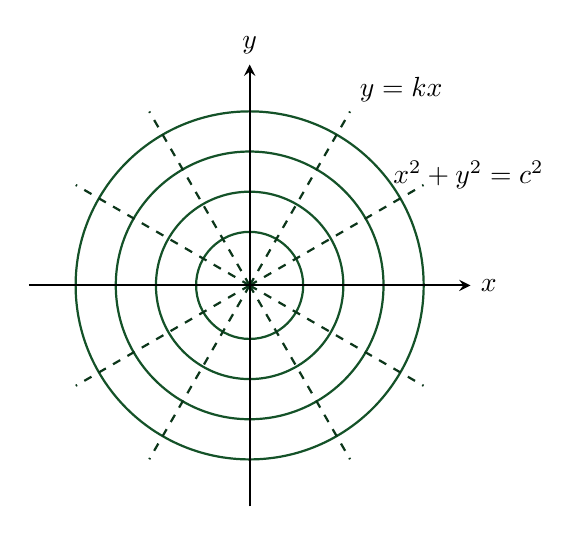
\begin{tikzpicture}[scale=0.85]
    % Concentric Circles
    \foreach \r in {0.8, 1.4, 2.0, 2.6} {
        \draw[AcademicGreen, thick] (0,0) circle (\r);
    }
    % Orthogonal Lines
    \foreach \angle in {0, 30, 60, 90, 120, 150, 180, 210, 240, 270, 300, 330} {
        \draw[DarkGreen, dashed, thick] (0,0) -- (\angle:3.0);
    }
    % Axes
    \draw[->, >=stealth, thick] (-3.3,0) -- (3.3,0) node[right] {$x$};
    \draw[->, >=stealth, thick] (0,-3.3) -- (0,3.3) node[above] {$y$};
    \node[anchor=north west] at (2,2) {$x^2+y^2=c^2$};
    \node[anchor=south west] at (1.5,2.6) {$y=kx$};
\end{tikzpicture}
\end{center}

\vspace{0.3cm}
\begin{tcolorbox}[greenbox]
    \textbf{\textcolor{AcademicGreen}{Example 2:}} Find the orthogonal trajectories of $y = cx^2$.
    
    \vspace{0.15cm}
    \noindent\textbf{Solution:} Differentiating $y = cx^2 \implies \frac{dy}{dx} = 2cx$.
    Since $c = \frac{y}{x^2}$, we get $\frac{dy}{dx} = 2\left(\frac{y}{x^2}\right)x = \frac{2y}{x}$.
    
    \noindent Replacing $\frac{dy}{dx}$ by $-\frac{dx}{dy}$:
    \[
    \frac{dy}{dx} = -\frac{x}{2y} \implies 2y \, dy + x \, dx = 0
    \]
    Integrating:
    \[
    y^2 + \frac{x^2}{2} = k_0 \implies x^2 + 2y^2 = k \quad \text{\textbf{Ans.}}
    \]
\end{tcolorbox}

\vspace{0.2cm}
\noindent\textbf{Exercise (S.L. Ross P.75):} Find a family of oblique trajectories of the family of straight lines $y = cx$ at an angle $\alpha = 45^\circ$.

\newpage

% ==========================================
% PAGE 8 (Corresponding to Image 8)
% ==========================================
\Heading{Higher Order Linear Differential Equations:}
A linear ordinary differential equation (LODE) of order $n$ in the dependent variable $y$ and independent variable $x$ is an equation that can be expressed as:
\begin{equation}
    a_0(x)\frac{d^n y}{dx^n} + a_1(x)\frac{d^{n-1}y}{dx^{n-1}} + \dots + a_{n-1}(x)\frac{dy}{dx} + a_n(x)y = F(x) \quad \text{--- (1)} \label{eq:lode_nonhomo}
\end{equation}
where $a_0(x) \neq 0$.

\vspace{0.15cm}
\noindent We assume that $a_0, a_1, \dots, a_n$ are continuous on an interval $a \le x \le b$ and $a_0(x) \neq 0$ for all $x \in [a,b]$.
The function $F(x)$ is called the \textbf{non-homogeneous term}.

\vspace{0.2cm}
\noindent If $F(x) = 0$, then equation \eqref{eq:lode_nonhomo} reduces to:
\begin{equation}
    a_0(x)\frac{d^n y}{dx^n} + a_1(x)\frac{d^{n-1}y}{dx^{n-1}} + \dots + a_{n-1}(x)\frac{dy}{dx} + a_n(x)y = 0 \quad \text{--- (2)} \label{eq:lode_homo}
\end{equation}
and is called a \textbf{homogeneous linear differential equation}.

\vspace{0.3cm}
\begin{tcolorbox}[theorembox, title=Existence and Uniqueness Theorem]
    Let $x_0$ be any point on $a \le x \le b$ and let $c_0, c_1, \dots, c_{n-1}$ be $n$ arbitrary constants.
    Then there exists a \textbf{unique solution} $f(x)$ of equation \eqref{eq:lode_nonhomo} satisfying the initial conditions:
    \[
    f(x_0) = c_0, \quad f'(x_0) = c_1, \quad \dots, \quad f^{(n-1)}(x_0) = c_{n-1}
    \]
    which is defined throughout $a \le x \le b$.
\end{tcolorbox}

\vspace{0.2cm}
\noindent\textbf{Note:} If $f$ is a solution of the homogeneous equation \eqref{eq:lode_homo} with $f(x_0) = 0, f'(x_0) = 0, \dots, f^{(n-1)}(x_0) = 0$, then $f(x) = 0$ identically on $a \le x \le b$.

\Heading{Linear Combination and General Solution:}

\noindent\textbf{Definition (Linear Combination):} If $f_1, f_2, \dots, f_m$ are $m$ functions and $c_1, c_2, \dots, c_m$ are $m$ constants, then the expression:
\[
c_1 f_1 + c_2 f_2 + \dots + c_m f_m
\]
is called a \textbf{linear combination} of $f_1, f_2, \dots, f_m$.

\vspace{0.2cm}
\noindent\textbf{Property:} If $f_1, f_2, \dots, f_m$ are $m$ solutions of homogeneous DE \eqref{eq:lode_homo}, then any linear combination $c_1 f_1 + c_2 f_2 + \dots + c_m f_m$ is also a solution of \eqref{eq:lode_homo}.

\vspace{0.3cm}
\begin{tcolorbox}[theorembox, title=Fundamental Theorem of Homogeneous LODEs]
    The $n^{\text{th}}$ order homogeneous linear DE \eqref{eq:lode_homo} always possesses $n$ linearly independent solutions.
    
    \vspace{0.15cm}
    \noindent Furthermore, if $f_1, f_2, \dots, f_n$ are $n$ linearly independent solutions of \eqref{eq:lode_homo}, then \textbf{every solution} of \eqref{eq:lode_homo} can be expressed as a linear combination:
    \[
    c_1 f_1 + c_2 f_2 + \dots + c_n f_n
    \]
    by a proper choice of constants $c_1, c_2, \dots, c_n$.
\end{tcolorbox}

\vspace{0.3cm}
\noindent\textbf{General Solution:} If $f_1, f_2, \dots, f_n$ are $n$ linearly independent solutions of \eqref{eq:lode_homo} on $a \le x \le b$, then:
\[
f(x) = c_1 f_1(x) + c_2 f_2(x) + \dots + c_n f_n(x)
\]
(where $c_1, c_2, \dots, c_n$ are arbitrary constants) is called the \textbf{general solution} of \eqref{eq:lode_homo}.

\vspace{3cm}

\begin{center}
    {\large\bfseries\textcolor{AcademicGreen}{The Wronskian}} \\[0.2cm]
    \vspace{0.3cm}
\end{center}
Let $f_1, f_2, \dots, f_n$ be $n$ real functions, each having at least $n-1$ derivatives on $a \le x \le b$. The determinant:
\[
W(f_1, f_2, \dots, f_n) = 
\begin{vmatrix} 
f_1 & f_2 & \dots & f_n \\ 
f_1' & f_2' & \dots & f_n' \\ 
\vdots & \vdots & \ddots & \vdots \\ 
f_1^{(n-1)} & f_2^{(n-1)} & \dots & f_n^{(n-1)} 
\end{vmatrix}
\]
is called the \textbf{Wronskian} of the functions $f_1, f_2, \dots, f_n$.

\vspace{0.15cm}
\noindent If the Wronskian $W(f_1, f_2, \dots, f_n) \neq 0$ for at least one point on $a \le x \le b$, then the functions are \textbf{linearly independent}.

\vspace{0.3cm}
\begin{tcolorbox}[greenbox]
    \textbf{\textcolor{AcademicGreen}{Example:}} Show that the solutions $e^x$, $e^{-x}$, and $e^{2x}$ of the DE
    \[
    \frac{d^3 y}{dx^3} - 2\frac{d^2 y}{dx^2} - \frac{dy}{dx} + 2y = 0
    \]
    are linearly independent.
    
    \vspace{0.15cm}
    \noindent\textbf{Solution:} Evaluating the Wronskian of $e^x, e^{-x}, e^{2x}$:
    \[
    W(e^x, e^{-x}, e^{2x}) = 
    \begin{vmatrix} 
    e^x & e^{-x} & e^{2x} \\ 
    e^x & -e^{-x} & 2e^{2x} \\ 
    e^x & e^{-x} & 4e^{2x} 
    \end{vmatrix}
    \]
    Factoring out $e^x, e^{-x}, e^{2x}$ from columns 1, 2, and 3:
    \[
    W = (e^x)(e^{-x})(e^{2x}) 
    \begin{vmatrix} 
    1 & 1 & 1 \\ 
    1 & -1 & 2 \\ 
    1 & 1 & 4 
    \end{vmatrix}
    \]
    \[
    = e^{2x} \left[ 1(-4 - 2) - 1(4 - 2) + 1(1 + 1) \right] = e^{2x} (-6 - 2 + 2) = -6 e^{2x} \neq 0 \quad \forall x \in \mathbb{R}
    \]
    Thus, since $W(e^x, e^{-x}, e^{2x}) \neq 0$ for all real values of $x$, $e^x, e^{-x}, e^{2x}$ are linearly independent solutions of the given differential equation on every real interval.
\end{tcolorbox}




\end{document}